% Generado por analysis/src/tablas/figuras_tex.py — no editar a mano.
\begin{figure*}[!tbp]
\centering
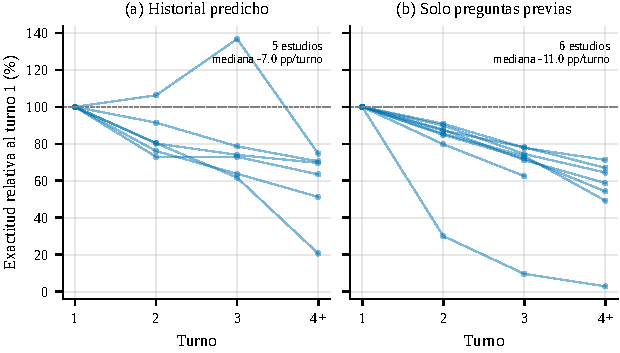
\includegraphics[width=4.14in,height=0.85\textheight,keepaspectratio]{pi5_degradacion}
\caption{Degradación de la exactitud a lo largo de los turnos (sistema propuesto, normalizada al turno 1; turnos $\geq$ 4 agrupados en «4+»), separada por el tipo de historial usado en la evaluación: (a) historial predicho; (b) solo preguntas previas. Valores por turno extraídos de las tablas de cada estudio y verificados en la página citada. Sin curvas con al menos tres turnos para: historial gold, no reportado. Los grupos de turno contienen preguntas distintas, por lo que la pendiente mezcla profundidad y dificultad; las pendientes no se agrupan entre estratos.}
\label{fig:pi5_degradacion}
\end{figure*}
